\documentclass[a4paper,12pt]{article}

% Pacotes essenciais
\usepackage[utf8]{inputenc}
\usepackage[T1]{fontenc}
\usepackage[brazil]{babel}
\usepackage{amsmath, amssymb}
\usepackage{graphicx}
\usepackage{booktabs}
\usepackage{caption}
\usepackage{siunitx}
\usepackage{geometry}
\geometry{a4paper, margin=1in}

\title{Relatório Detalhado (Atividade 7): \\ Análise da Transformação Não-Linear Pós-PCA}
\author{Lucas José Lemos Braz (Análise gerada por IA)}
\date{Agosto, 2025}

\begin{document}

\maketitle

\section{Introdução}

A Atividade 7 introduz um passo adicional de refinamento no pipeline de pré-processamento. Após validar a eficácia da redução de dimensionalidade com PCA, esta etapa investiga se uma \textbf{transformação não-linear} subsequente pode extrair ainda mais desempenho dos classificadores. 

O objetivo é testar a hipótese de que, ao forçar a distribuição de cada componente principal a se aproximar de uma distribuição Gaussiana, podemos melhorar a separabilidade das classes. Para isso, o seguinte pipeline foi implementado e avaliado: \texttt{PCA (redução) -> Box-Cox -> Z-Score}.

\section{Metodologia}

O protocolo experimental seguiu o mesmo rigor das atividades anteriores, com a adição da transformação Box-Cox no fluxo de pré-processamento para cada uma das 50 repetições.

\subsection{Pipeline de Pré-processamento}

\begin{enumerate}
    \item \textbf{Divisão e Redução com PCA:} Os dados foram divididos em treino/teste, e o PCA (com \(q=79\)) foi ajustado no conjunto de treino e aplicado a ambos os conjuntos. 
    
    \item \textbf{Transformação Box-Cox:}
    \begin{itemize}
        \item \textbf{Ajuste:} Para cada um dos 79 componentes principais, o parâmetro \(\lambda\) da transformação Box-Cox foi estimado \emph{exclusivamente} sobre os dados de treino, buscando maximizar a log-verossimilhança da distribuição resultante.
        \item \textbf{Garantia de Positividade:} Como a transformação Box-Cox exige dados estritamente positivos, e os componentes principais são centrados em zero, um deslocamento (\emph{shift}) foi calculado a partir do valor mínimo de cada componente no treino e adicionado a todos os dados antes da transformação.
        \item \textbf{Aplicação:} Os parâmetros \(\lambda\) e \emph{shift} de cada componente, aprendidos no treino, foram usados para transformar ambos os conjuntos (treino e teste).
    \end{itemize}
    
    \item \textbf{Normalização Z-Score Final:} Após a transformação não-linear, uma normalização Z-Score foi ajustada nos dados de treino e aplicada a ambos os conjuntos. Isso garante que as características de entrada para os classificadores tenham média 0 e desvio padrão 1, condição ideal para otimizadores baseados em gradiente.
\end{enumerate}

\subsection{Hipótese e Análise Crítica}

\noindent\textbf{A Hipótese Central:} Modelos de classificação, especialmente os lineares, performam otimamente quando as características de entrada seguem uma distribuição Gaussiana. Portanto, aplicar a transformação Box-Cox para \"gaussianizar\" os componentes principais deveria facilitar a tarefa de separação das classes. 

\noindent\textbf{Análise Crítica (O Contraponto Teórico):} Esta hipótese, embora geralmente válida, pode não se aplicar neste contexto. Pelo \textbf{Teorema do Limite Central}, a soma de muitas variáveis aleatórias tende a uma distribuição Gaussiana. Como os componentes principais são combinações lineares de centenas de pixels, é provável que os componentes mais significativos \textbf{já sejam naturalmente próximos de uma distribuição normal}. 

Sendo assim, a expectativa real é que a aplicação de uma segunda e potente transformação de normalização (Box-Cox) seja desnecessária e possa até \textbf{distorcer prejudicialmente} uma geometria de dados que já era favorável, além de adicionar custo computacional.

\section{Resultados e Discussão}

Os resultados empíricos confirmaram a análise crítica em detrimento da hipótese inicial.

\begin{figure}[h!]
  \centering
  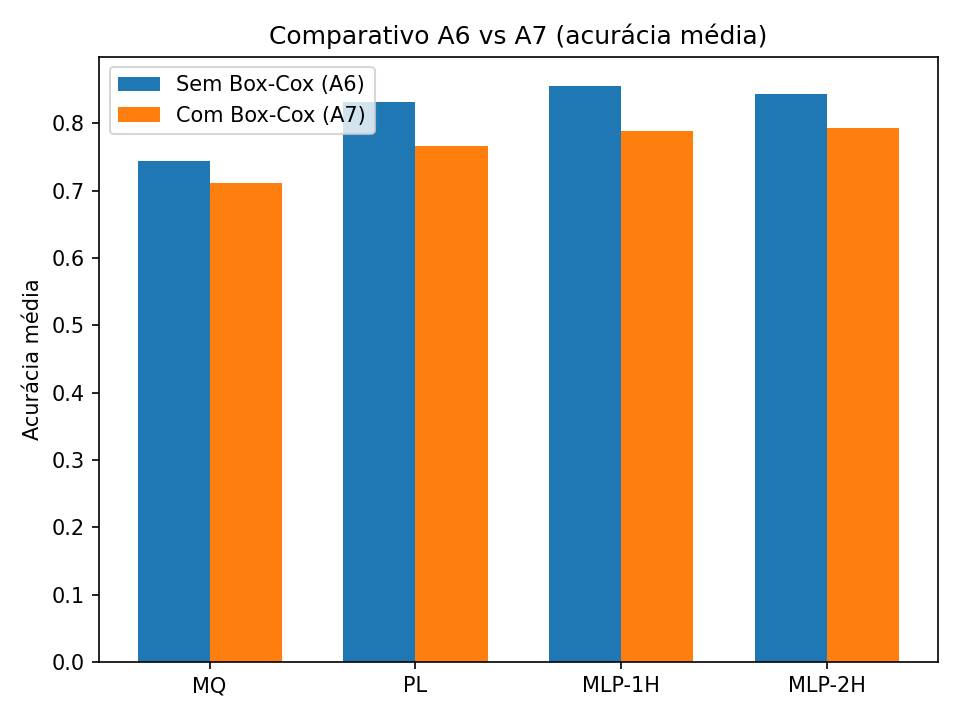
\includegraphics[width=0.8\textwidth]{../results/TC2/comparativo_A7_acc.png}
  \caption{Comparativo de acurácia média entre a Atividade 6 (PCA com \(q=79\)) e a Atividade 7 (PCA + Box-Cox). Observa-se uma degradação sistemática e consistente no desempenho de \textbf{todos} os classificadores após a aplicação da transformação Box-Cox.}
  \label{fig:comparativo_a7}
\end{figure}

Como ilustrado na Figura~\ref{fig:comparativo_a7}, a adição da transformação Box-Cox ao pipeline resultou em uma \textbf{piora sistemática da acurácia} para todos os quatro classificadores. O desempenho, que havia sido recuperado e até melhorado com a redução de dimensionalidade na Atividade 6, foi novamente degradado.

Esta evidência sugere fortemente que os componentes principais já formavam um espaço de características bem-comportado e com alto poder de separação. A transformação não-linear de Box-Cox, ao invés de ajudar, introduziu uma distorção que tornou as classes menos separáveis, prejudicando a performance dos modelos. Além disso, o custo computacional para estimar os parâmetros \(\lambda\) em cada repetição, embora modesto, não trouxe qualquer benefício que o justificasse.

\section{Conclusão}

A Atividade 7 serve como uma importante lição sobre a aplicação criteriosa de técnicas de pré-processamento. Ela demonstra que \"boas práticas\" aplicadas de forma isolada ou cega, sem considerar as propriedades dos dados em cada etapa do pipeline, podem ser contraproducentes. 

Neste caso, a tentativa de \"gaussianizar\" características que provavelmente já eram aproximadamente gaussianas resultou em uma piora de desempenho. A conclusão é clara: para este problema, o pipeline ideal consiste na redução de dimensionalidade com PCA seguida de uma simples normalização (como Z-Score ou Min-Max), e a transformação de Box-Cox deve ser descartada.

\end{document}
